\begin{wrapfigure}{l}{0.45\textwidth}
  \scalebox{0.9}{
    \hspace{-8pt}
    \begin{tabular}{m{1pt}c}
      \multirow{2}*{
        \rotatebox{90}{\tiny magnitude $w_i$}
      }
      \hspace{2pt}
      &
      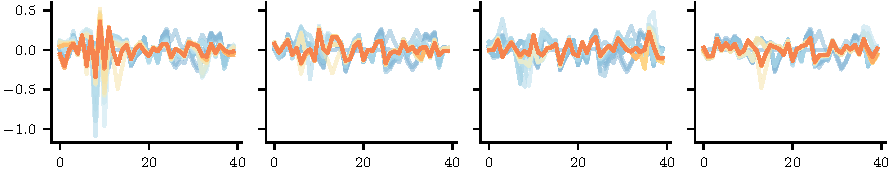
\includegraphics[width=\linewidth]{figures/multi-neuron/10erf_alg4_subset4.pdf} \\
      &
      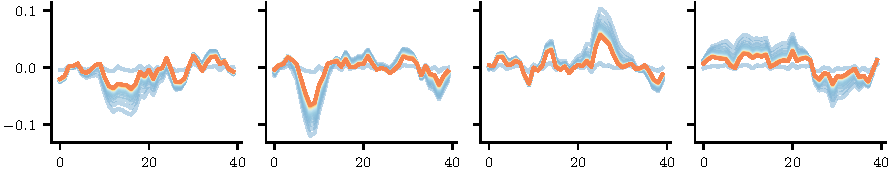
\includegraphics[width=\linewidth]{figures/multi-neuron/10erf_alg30_subset4.pdf}  \\
      \noalign{\vskip -4pt}
      &\hspace{18pt}\tiny dimension $i$ of weight $\mathbf{w}$
    \end{tabular}
  }
  \caption{
    具有可学习的第二层权重的多神经元模型 (\labelcref{item:many-neuron-model})
    的感受野,$N=40$,$K=10$。
    (\textbf{上图}) 来自一个使用sigmoid激活函数的模型的4个随机感受野子集,
    该模型在$\texttt{Kur(4)}$上训练(正的超额峰度为$3.28$)。
    正如命题~\labelcref{thm:localization}所预测的,
    这些感受野\emph{不是}局部化的,而表现为高频振荡。
    (\textbf{下图}) 来自一个使用ReLU激活函数的模型的4个随机感受野子集,
    该模型在$\texttt{Kur(30)}$上训练(负的超额峰度为$-1.17$)。
    感受野是局部化的(\textbf{左三})或表现为低频振荡(\textbf{右})。
    \emph{参见 \cref{sec:extensions} 以获取详细说明。}
  }
  \label{fig:multi-neuron}
\end{wrapfigure}
